\documentclass[a4paper, twoside]{report}

\usepackage[english]{babel}
\usepackage[utf8x]{inputenc}
\usepackage[T1]{fontenc}
\usepackage{listings}
\usepackage{hyperref}
\hypersetup{colorlinks=false}
\usepackage{lscape}
\usepackage{subfigure}
\usepackage{amsmath}
\usepackage{graphicx}
\usepackage[colorinlistoftodos]{todonotes}
\newcommand{\subsubsubsection}[1]{\paragraph{#1}\mbox{}\\}
\setcounter{secnumdepth}{4}
\setcounter{tocdepth}{4}
%% Sets page size and margins
\usepackage[a4paper,top=3cm,bottom=2cm,left=3cm,right=3cm,marginparwidth=1.75cm]{geometry}
\providecommand{\keywords}[1]{\textbf{\textit{Index terms---}} #1}

\title{Upgrading the HEP-Frame Scheduling Dependency Graph To support Conditional Task Graphs }
\author{José Pedro Moreira Resende}

\begin{document}
\begin{titlepage}

\newcommand{\HRule}{\rule{\linewidth}{0.5mm}} % Defines a new command for the horizontal lines, change thickness here

%----------------------------------------------------------------------------------------
%	LOGO SECTION
%----------------------------------------------------------------------------------------


\includegraphics[width=6cm]{title/logo.png} % Include a department/university logo - this will require the graphicx package

%----------------------------------------------------------------------------------------

\center % Center everything on the page

%----------------------------------------------------------------------------------------
%	HEADING SECTIONS
%----------------------------------------------------------------------------------------
\quad\\[1.5cm]
%\textsc{\LARGE MSc Thesis}\\[1.5cm] % Name of your university/college
\textsc{\Large University of Minho}\\[0.5cm] % Major heading such as course name
\textsc{\large Department of Informatic}\\[1.5cm] % Minor heading such as course title

%----------------------------------------------------------------------------------------
%	TITLE SECTION
%----------------------------------------------------------------------------------------
\makeatletter
\HRule \\[0.4cm]
{ \huge \bfseries \@title}\\[0.4cm] % Title of your document
\HRule \\[1.5cm]

%----------------------------------------------------------------------------------------
%	AUTHOR SECTION
%----------------------------------------------------------------------------------------

\begin{minipage}{0.4\textwidth}
\begin{flushleft} \large
\emph{Author:}\\
\@author % Your name
\end{flushleft}
\end{minipage}
~
\begin{minipage}{0.4\textwidth}
\begin{flushright} \large
\emph{Supervisor:} \\
Prof. André Martins Pereira
% Uncomment the following lines if there's a co-supervisor
%\\[1.2em] % Supervisor's Name
%\emph{Co-Supervisor:} \\
%Dr. Adam Smith % second marker's name
\end{flushright}
\end{minipage}\\[5cm]
\makeatother


%----------------------------------------------------------------------------------------
%	DATE SECTION
%----------------------------------------------------------------------------------------

{\large A thesis submitted for the degree of}\\[0.5cm]
{\large \emph{MSc Software Engineering}}\\[0.5cm]
{\large \today}\\[2cm] % Date, change the \today to a set date if you want to be precise

\vfill % Fill the rest of the page with whitespace

\end{titlepage}


\begin{abstract}
Scientists often develop applications to analyse large datasets and process raw data into useful information with scientific value. These applications are typically structured as a sequence of tasks in a pipeline of actions, where data can be modified at each pipeline stage, filtered out and/or output as a result. The elements that are filtered out are not processed by the next tasks in the pipeline. Actions often vary from intensive computing tasks to simple evaluations that may discard irrelevant data.
\par The increasing complexity of the algorithms and the size of the datasets to be analyzed makes this type of problem computationally intensive and hard to end in a timely manner. Since these applications are usually developed by the end-user, a non-programming expert working in a scientific domain, such as physics or chemistry, the overall performance of the code execution may even be more affected. This is due to the fact that scientists focus their programming effort in the correctness of the algorithm implementation and the time to obtain results, leaving behind issues like the performance of the resulting code (and associated data structures) and its execution on specific hardware platforms.
\par Current compute servers are inherently very parallel, supporting several forms of parallel execution of code: from simultaneous execution of several tasks (on an increasing number of physical cores or processing units, PUs) to the execution of the same task (or sets of instructions) on different data elements (aka known as vector computing). A framework was deployed to aid scientists to develop scientific applications that are based on a pipeline of actions (that may be discarded along its path) applied to a very large dataset, and to efficiently manage their code execution in homogeneous and heterogeneous servers: the Highly Efficient Pipeline Framework, HEP-Frame.
\par The current HEP-Frame version only supports one type of decision at the end of each action or pipeline stage: either the outcome of the action satisfies a given criterium (or set of criteria) and follows the pipeline path, or fails and the data element is no longer processes, i.e., is discarded. However, some scientific applications, such as particle analysis, require that the decision on some pipeline stages may lead to different alternative solutions, namely different pipeline paths. This issue will be addressed as conditional task graphs.

\end{abstract}

\renewcommand{\abstractname}{Resumo}
\begin{abstract}
  resumo
\end{abstract}


\clearpage % Start a new page

\tableofcontents
\listoffigures
\listoftables

\chapter{Introduction}

\section 

\chapter{State of the art}



\subsection{Pequena intro a existencia de HW cada vez mais complexo e ao sw necessario para usar eficientemente}

\subsection{HW}
\subsubsection{Multicore}
\subsubsubsection{Descrever em detalhe todas as caracteristicas que sao importantes como multiplos cores, caches, vectorizacao, etc}
\subsubsubsection{Intel/AMD}
\subsubsection{Manycore}
\subsubsubsection{Descrever em detalhe todas as caracteristicas que sao importantes KNL, ver slides de AA}
\subsubsubsection{ARM}
\subsection{Pipelines condicionais *em detalhe e com imagens (e dizer qu eas tarefas sao irregulares)}
\subsection{SW}
\subsubsection{tudo o que precises ou que exista de carater geral desde boost threads, openMP, mpi, tbb, etc}
\subsubsection{tudo o que procuraste (descrever o que e e o proposito, de escalonadores, list schedulers (e importante ter alguma coisa e provar que nao e util para o nosso problema, ferammentas DAG, etc, uteis para nos }
\subsubsection{Se calhar uma secao so para falar de grafos (algoritmos para construir e manipular so os que poderao ser uteis)}
\chapter{Work Plan}
\section{Proposed approach}
\subsection{Ja detalhes concretos de como se deveria estruturar e implementar as coisas (falar do que ja esta feito ou esta a ser feito)}
At this point we have a preprocessor capable of parse the source code, read all the tasks defined by the user and generate the condiditional graph. This is a simple context based parser that takes in return value of a function that can be considered a step on the pipeline and 
\subsection{Definicao do prototipo das tarefas (restricoes e codigo}
\subsection{qual o pre processamento e como o fazer concretamente (tudo desde criar Dag, se as dependencias sao validas,etc}
\subsection{qual a abordagem a tomar para o escalonador}
\subsubsection{ideias, imagens, como devera ser dividida a carga}
\subsubsection{branch prediction}
\subsubsection{definicao ja dos requisitos que o benchmark sintetico tera}

\chapter{Preliminary work}
Some work was developed during this initial stage of the thesis work, namely on the research and implementation of different graphs and strategies to validate them.
This chapter includes a explanation for the type of graphs that may be used, alongside their key characteristics, concurrency models and the different components mentioned in the previous chapters.

\section{Graph Theory}

Graph theory classifies different graphs by their properties and characteristics. Some of the more relevant types of graphs for this dissertation are: 
\begin{itemize}
    \item Complete graph: every pair of distinct vertices is connected by a unique edge;
    \item Directed graph: where edges have a direction associated with them;
    \item Acyclic graph: a finite directed graph with no directed cycles;
    \item Strongly connected graph: when every vertex is reachable from every other vertex;
    \item Supergraph:  formed by adding vertices, edges, or both to a given graph;
    \item Component (or connected component): vertices connected to each other by paths and which is connected to no additional vertices in the supergraph;
    \item Subgraph another graph formed from a subset of the vertices and edges;
    \item Dependency graph representation dependencies of several objects towards each other; if a dependency graph does not have any circular dependencies, it forms a Direct Acyclic graph;
    \item Task graph tasks are vertices with edges between them representing dependencies between tasks.
\end{itemize}

As referred in the previous chapters, these graphs are required to represent the task execution-order (addressed in this work as TEG).
% was understood in the previous chapters that we need graphs to represent the task execution-order -- \textbf{TEG}.

A suitable TEG graph needs to respect the following properties: 
\begin{enumerate}
    \item Must represent tasks and paths connecting tasks (vertices and edges), where the edges have a direction associated with them (directed graph);
    \item Must have one start vertex(task) and always reach one end vertex(task);
    \item Must represent the weight of a task;
    \item Must represent dependencies between tasks;
    \item Each task may be executed at most once (acyclic graph);
    \item May have an hierarchical representation with subgraphs;
    \item Subgraphs may be strongly connected and complete graph;
    \item Must support multiple paths between the starting and the ending   vertices.
\end{enumerate}{}


Following these criteria the previous graph types can be classified as \textit{suitable}, \textit{maybe} or \textit{not suitable} for TEG, as shown in table \ref{tab:teg}.

\begin{table}[tbh!]
\begin{center}
\begin{tabular}{l|l}
Complete graph                     & \ding{55}    \\ \hline
Directed  graph                    & \ding{51} \\ \hline
Acyclic graph                      & ?         \\ \hline
Strongly connected graph           & ?         \\ \hline
Supergraph                         & \ding{55} \\ \hline
Component (or connected componect) & \ding{55} \\ \hline
Subgraph                           & \ding{51} \\ \hline
Dependency graph                   & \ding{51}\\ \hline
Task graph                         & \ding{51}     
\end{tabular}
\end{center}
\caption{Suitability of the representation of a task execution-order in different graphs.}
\label{tab:teg}
\end{table}


\section{Pre-processor}

\par A preprocessor  capable of parsing a C/C++ source file, analyse it and generate the corresponding conditional graph has already started development. 
This is a simple parser written in \textit{python} using this language builtin \textit{regular expression} engine. With the use of regular expressions the parser can understand when it is inside of a function, using a reference counter of the bracket symbol, and increasing or decreasing this counter when a \textit{{} or a \textit{}} is found. Together with this we can also find out if a given function belongs to the user pipeline analysing the function return type and signature.
The return values of each function can be identified and considered the next step of the pipeline, thus creating the graph based on them. It is also required to create a syntactic fail node for when a stage in the pipeline fails and we want to halt all the computation for this data-set and pass the execution to the next in line, allowing for the most efficient execution possible.

After creating the graph it is needed to save its state to disk for future loading, validation of correctness and as a intermediate structure that the scheduler is going to use to create a TEG. 
Different formats and ways to encode and save this graph were explored, including the language binary representation of the \textit{struct}, generic binary representation, domain-specific language and generic text formats. All these formats have trade-offs in speed and readability, but this being a dissertation as a goal to extend a framework that is supposed to be user-friendly, it was opted to go with the more readable and easier to analyse format, such as generic text formats. Within this type of format, it was concluded that the best options were JSON, YAML and XML, for they provide the better parser libraries and visualisation/editing tools. 
After some preliminary testing, XML was excluded for being too verbose and therefore infringing the requirements defined in the previous stage. JSON can be used as a YAML subset; therefore, it can be used in tools designed for booth formats. For all these reasons it was concluded that JSON is the best format to be used to encode our graph in a file that is going to be saved to disk and later used in some additional tasks.

\section{Graph validation}

Deadlocks and infinite loops can occur in a conditional pipeline, as the user has a high degree of freedom when defining it.

\begin{figure}[h]
\begin{center}
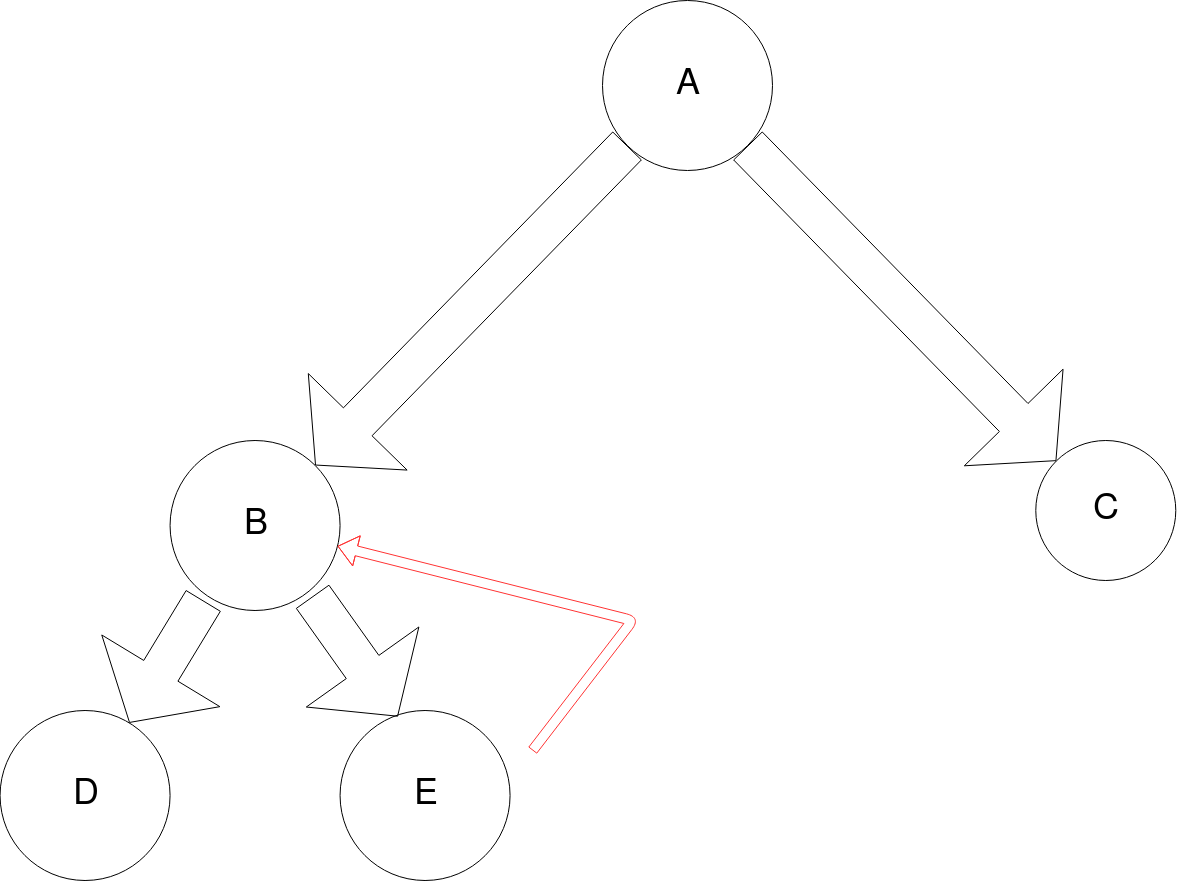
\includegraphics[width=10cm]{latex/img/CiclicGraph}
\end{center}
\caption{A tree-like graph representing possible execution flows among conditional propositions with a cycle (red arrow).}
\label{fig:graph}
\end{figure}

To prevent such cases an algorithm to analyse the graph to assess if a graph is acyclic should be used.
For instance, figure \ref{fig:graph} presents a graph that has a cycle that must be avoided.
For this the Depth First Search traversal, Tarjan's strongly connected components algorithm or Topological sorting algorithms can be used.

\section{Condition validation}
The graph should be able to contain conditional tasks to control the flow through the graph.
User coded conditions of the propositions must be validated to check if the condition is satisfiable.
In the case it is not satisfiable the proposition can remove or out right refuse to run the program and warn the user to change it.
The conditional pipeline can be considered as boolean satisfiable problem and a SAT solver should be used to validate these conditions.
The Boolean satisfiability problem also abbreviated to SATISFIABILITY or SAT is the problem of determining if a interpretation that satisfies a given boolean formula exists. 
SAT solver is the program that given a first order boolean formula (TRUE, FALSE, OR, AND, NOT)  solves this type of problems.
Boolean conditions that are not first order must be reduce to first order. For instance, if a condition (x>0) AND (A OR B) can be transformed in to C AND (A OR B). 


\section{Speculative execution/ concurrency model}
One common optimisation strategy used at the hardware level to improve the performance of conditional branches is branch prediction and speculative execution. It was already identified branch prediction may be a key component of the task scheduling strategy, as it allows subsequent tasks to be processed simultaneously with a current task without knowing its result yet. This should be considered when defining the graph to ensure that, through the analysis of this graph, every code execution with task dependencies, conditional paths, and branch prediction provides the correct results.
With this idea in mind it was tried to search for a concurrency model that could easily satisfy this kind of problem and end up finding for multithreading Posix threads, boost threads and the  actors model and for multi-processing async/await, MPI and CSP.
Probably most of the multithreading implementation will resort to Boost threads and/or Posix threads, but some of the speculative execution may be done through the use of the async/await paradigm.

\section{Synthetic test case}
A preliminary synthetic data analyses pipeline was developed in this phase, which emulates the type of conditional propositions that could benefit from the proposed schedular. This benchmark allows to abstract the development from more complex applications, making it easier and simple to implement and test new ideas that may come by as a possible way to speed up the user source code.

This type of program is characterized by irregular workload, which means that tasks have variable execution times within the same pipeline. These tasks can range from simple verification of integers to complex and/or compute intensive operations, such as matrix-matrix operations. To recreate correctly the workload this irregular behaviour must be replicated.
Using simulated data and computations, opposed to random process sleeps commonly using in synthetic scheduler benchmarking, will also help to get a better feel of real world performance for the proposed scheduler strategies. This will allow the creation of a standard group of tests from the most normal workload to the extreme edge cases to prove the robustness of this work.

To create a dataset that can be used a synthetic data block was created with the following structure:
\begin{lstlisting}
  std::vector<float> m_vector_float_a;
  std::vector<float> m_vector_float_b;
  std::vector<float> m_vector_float_c;

  std::vector<int> m_vector_int_a;
  std::vector<int> m_vector_int_b;
  std::vector<int> m_vector_int_c;

  std::vector<std::vector<int>> m_matrix_a;
  std::vector<std::vector<int>> m_matrix_b;
  std::vector<std::vector<int>> m_matrix_c;

  std::vector<std::vector<float>> m_matrix_float_a;
  std::vector<std::vector<float>> m_matrix_float_b;
  std::vector<std::vector<float>> m_matrix_float_c;

  int m_int_a{};
  int m_int_b{};
  int m_int_c{};

  float m_float_a;
  float m_float_b;
  float m_float_c;

  std::vector<int> m_list_ints;

  std::vector<float> m_list_floats;

\end{lstlisting}
A group of vectorial, single arithmetic operation and matrix-matrix operations can be described as:
\begin{lstlisting}
template <typename T>
void prod_matrix(std::vector<std::vector<T>> &a, std::vector<std::vector<T>> &b,
                 std::vector<std::vector<T>> &c) ;

template <typename T>
void dot_prod_matrix(std::vector<std::vector<T>> &a,
                     std::vector<std::vector<T>> &b,
                     std::vector<std::vector<T>> &c) ;

template <typename T>
bool is_positive(T number) ;

template <typename T>
void add(T &number) ;

template <typename T>
void filter_list(std::vector<T> &list, T number) ;
\end{lstlisting}

Using the C++ template system it is possible to quickly develop multiple generic functions over our Data structure. This way building a pipeline for proof-of-concept purposes can be done quickly and easily with most of the code being generate by the compiler.


\end{document}
